\begin{lemma}
The transmitted power in an optimal solution is non-decreasing with time whenever the receiver is \textit{on}.
\label{increasing_power}
\end{lemma}
\begin{proof}
We prove this by contradiction. The following two cases arise according to the receiver being \textit{on} or \textit{off}.

$Case1:$ Assume that the transmit power is $p_1$ from time $A$ to $B$ and then $p_2$ from $B$ to $C$ with $p_1>p_2$ and the receiver is \textit{on} throughout time $A$ to $C$ as shown in figure \ref{Lemma1}. In this case suppose we transmit at a power $p'=\dfrac{p_1(B-A)+p_2(C-B)}{C-A}$ then the number of bits transmitted would be more over the same time duration due to concavity of $g(p)$ as shown below.
\begin{align}
&g(p_1)\frac{B-A}{C-A}+g(p_2)\frac{C-B}{C-A} \le g(\frac{p_1(B-A)+p_2(C-B)}{C-A})
\\
&\implies g(p')(C-A)\ge g(p_1)(B-A)+g(p_2)(C-B)  
\end{align}
As we can transmit more number of bits during $C-A$ with power $p'$ we could save total transmition time since we would have lesser number of bits left to transmit after time $C$. Hence this case cannot be optimal.

$Case2:$ The receiver is \textit{off} for certain duration (say from $B$ to $C$) of time during $A$ to $D$ as shown in figure \ref{Lemma1}. The transmition power is $p_1$ from $A$ to $B$ and $p_2$ from $C$ to $D$. Now consider the case where keeping everything else intact we put the receiver \textit{off} from instant $A$ to $A+C-B$ and keep transmition from $A+C-B$ to $D$. This would always be feasible from the receiver point as energy with the receiver can only be non-decreasing with time. This scenario now boils down to $case-1$ from time $A+C-B$ to $D$ and hence cannot be optimal.
\end{proof}

\begin{figure}[htb]
\begin{minipage}[b]{0.48\linewidth}
  \centering
  \centerline{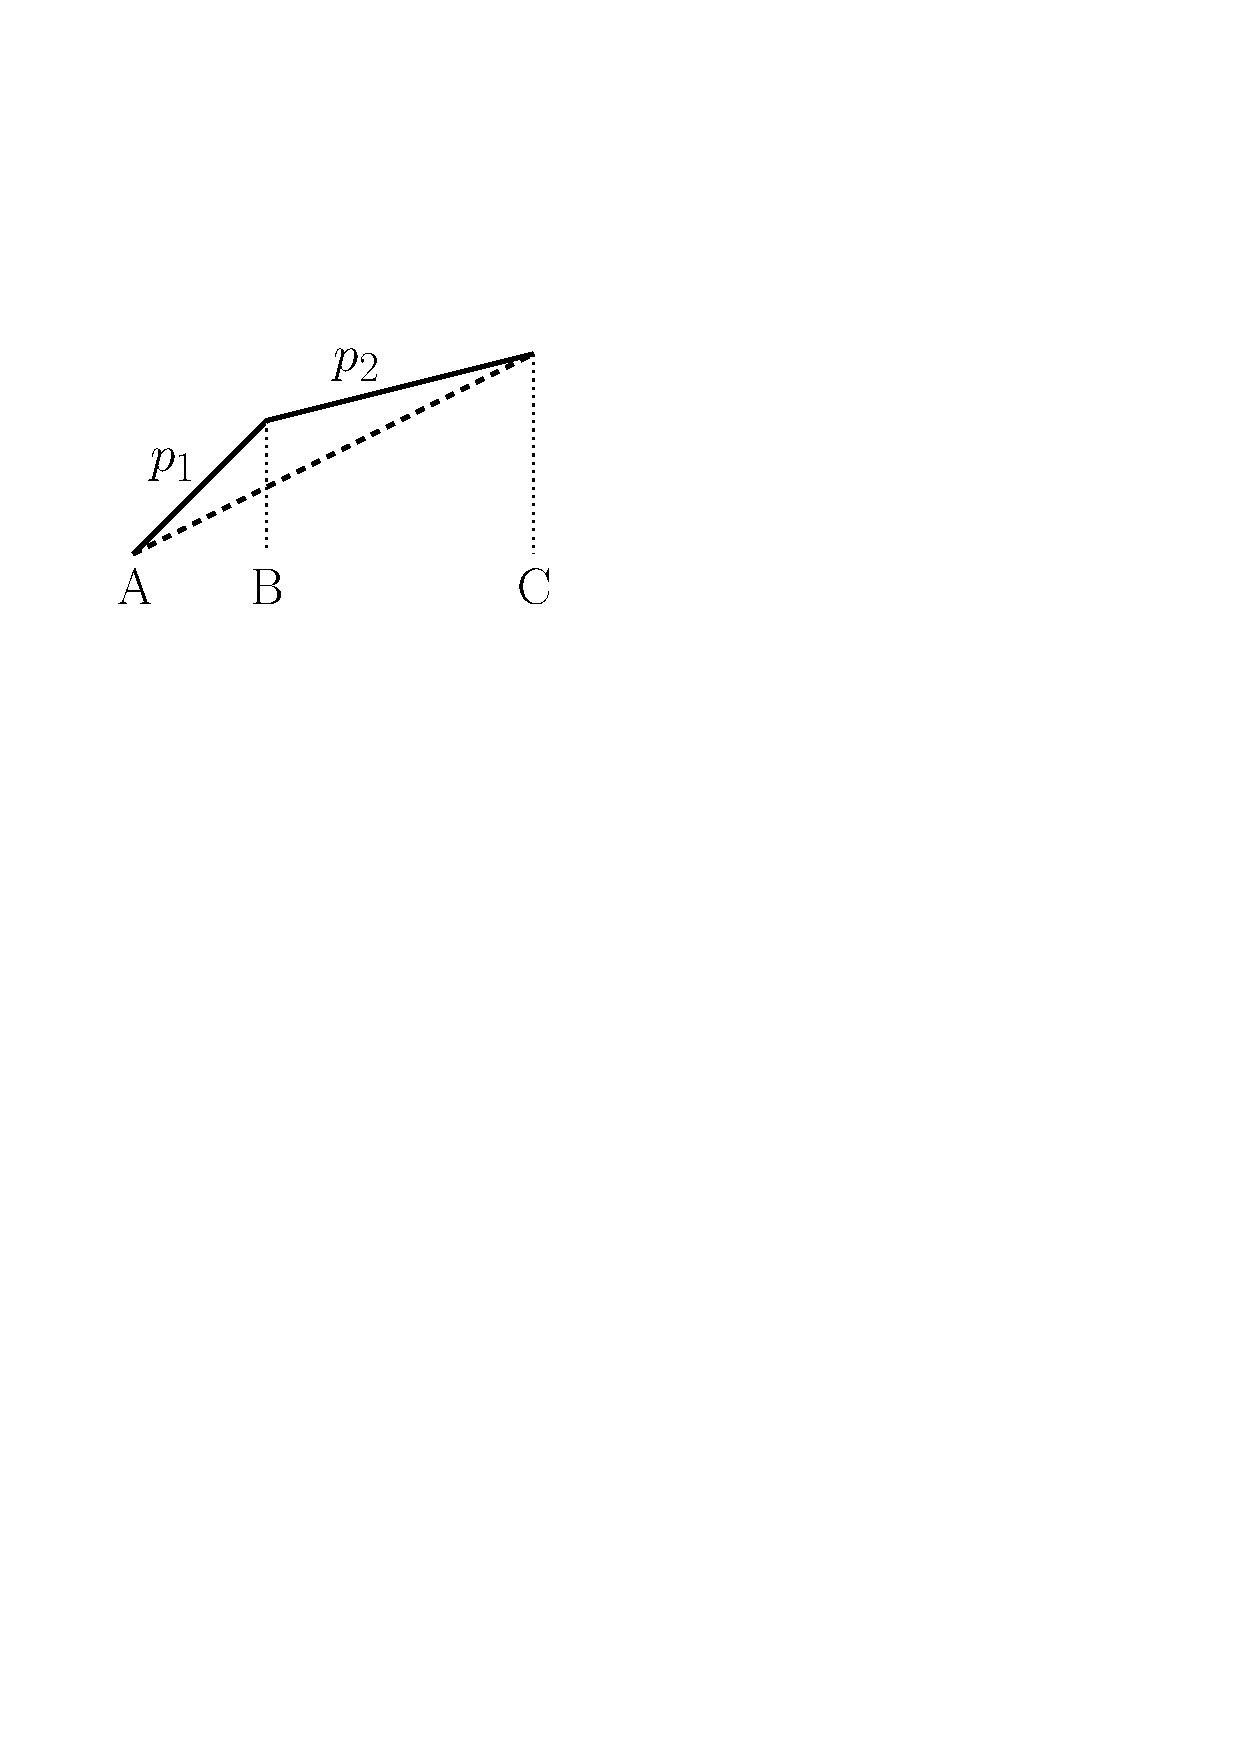
\includegraphics[width=4cm]{Lemma1_case1.pdf}}
\end{minipage}
\begin{minipage}[b]{0.48\linewidth}
  \centering
  \centerline{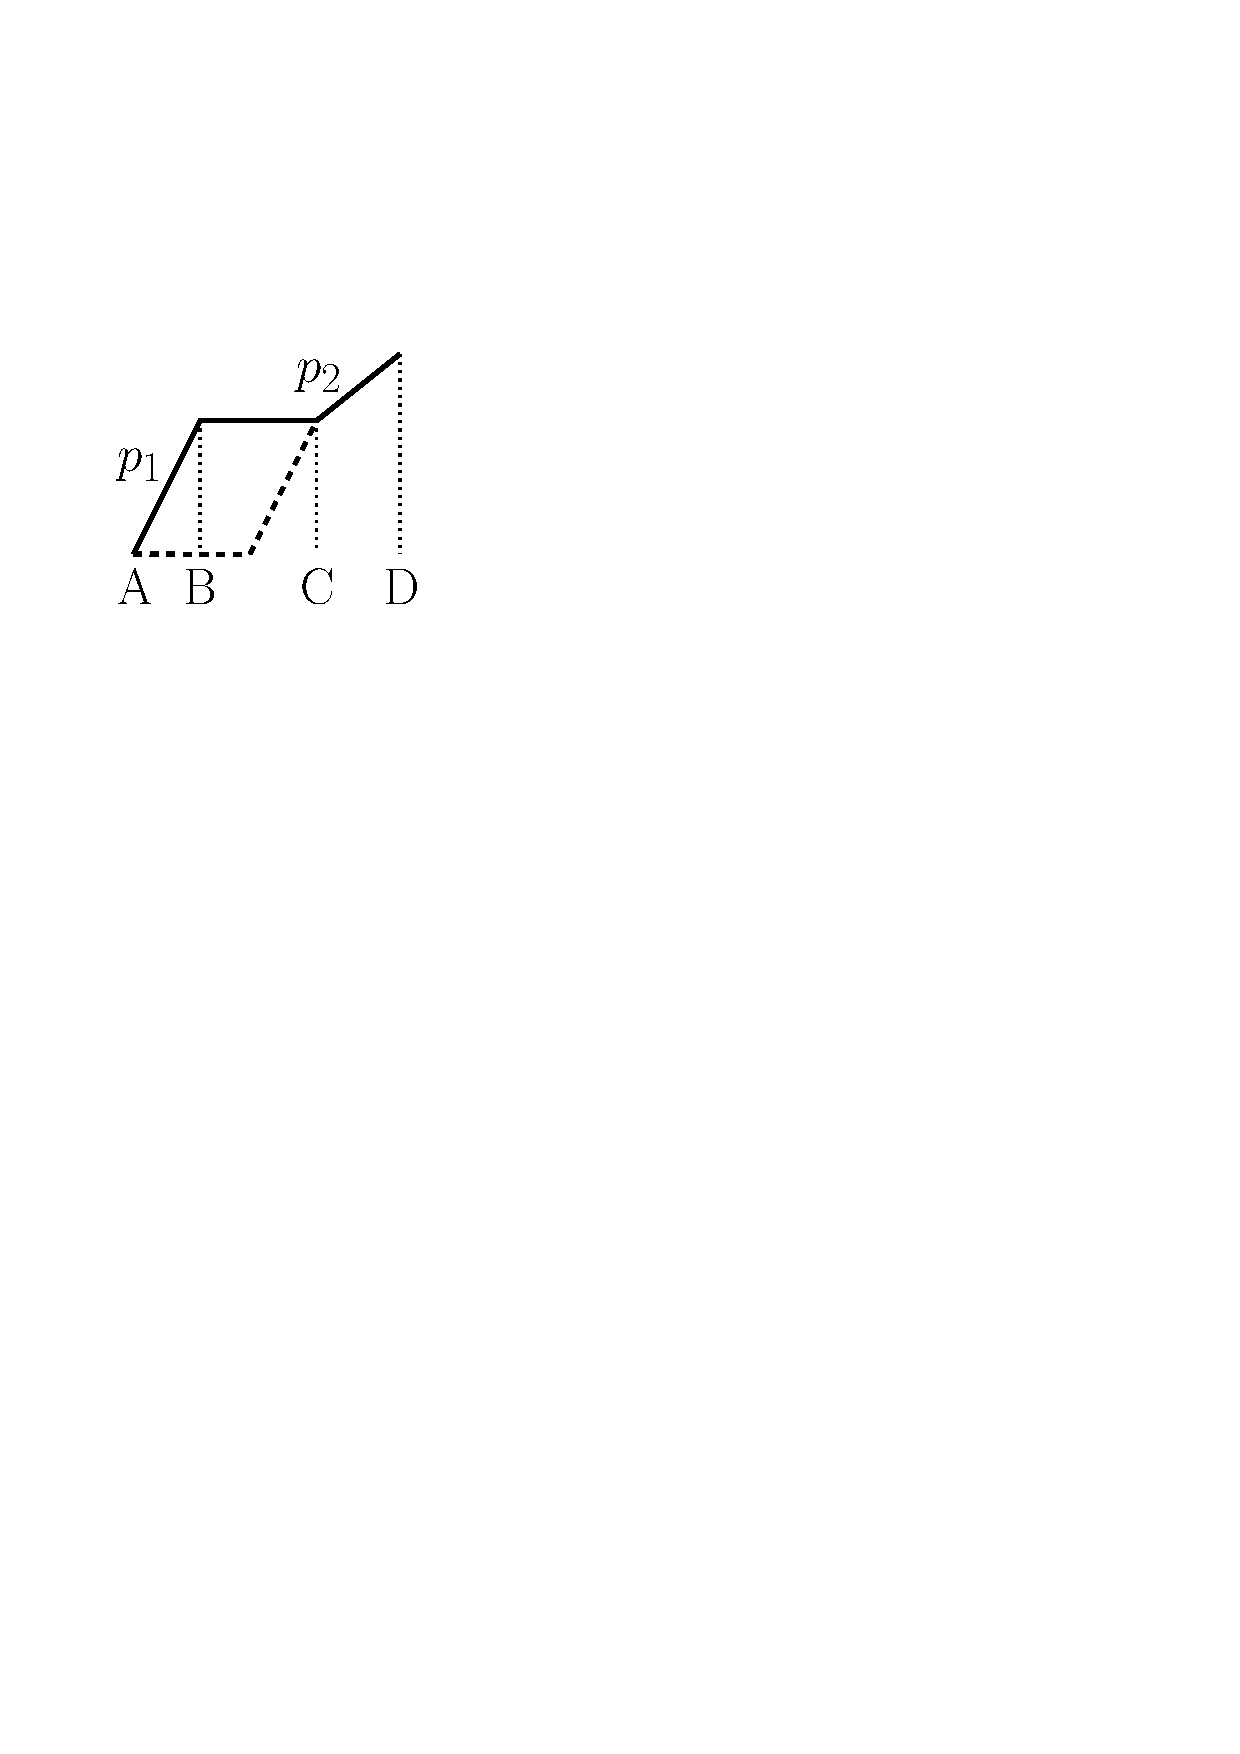
\includegraphics[width=4cm,height=25mm]{Lemma1_case2.pdf}}
\end{minipage}
\caption{Figure showing the two cases of Lemma 1, case 1[left] case2 [right] with $p_1>p_2$}
\label{Lemma1}
\end{figure}

\begin{lemma}
In an optimal solution once transmition has started the receiver is never \textit{off} until transmition is complete. \label{nobreaks}
\end{lemma}
\begin{proof}
This is equivalent to saying there is no-breaks during transmition in optimal solution. We again prove this by contradiction. Keeping intact Lemma \ref{increasing_power} the only case in which this can occur is the transmitter transmits with power $p_1$ from time $A$ to $B$ and then the receiver is \textit{off} from $B$ to $C$, again the transmitter is \textit{on} with power $p_2$ from time $C$ to $D$ with $p_1<p_2$ as shown in figure . Consider the case where we keep the receiver \textit{off} form time $A$ to $B'=A+C-B$. Now, a energy arrival can occur at the transmitter anywhere between $A$ to $D$. If there is no energy arrival then transmitting at a constant rate from $B'$ to $D$ would transmit more number of bits.

$case-1:$If the energy arrival is between $A$ and $B'$, then it can be easily seen that transmitting at a constant rate from $B'$ to $D$ would be better due to concavity of $g(p)$.

$case-2:$If the arrival is between $B'$ and $C$ (say $C'$), then it can be easily seen that transmitting at a same rate $p_1$ from $B'$ to $C'$ and  at a constant rate from $C'$ to $D$ would deliver more number of bits.(At worst case energy arrival occurring at $C$ would make this scenario transmit equal number of bits as the original scenario).

$case-3:$If there is an energy arrival from $C$ to $D$ (say $D'$), then transmitting at a constant power form $B'$ to $D'$ and then at same rate $p_2$ from $D'$ to $D$ would fetch more number of bits at the receiver.

Applying the above scenarios iteratively we could shift the receiver \textit{off} duration $C-B$ to the beginning of transmition and still at worst case transmit equal number of bits in same time duration. Hence having a break in-between transmition is always discouraged. We can also see that the optimal solution may not be unique.
\end{proof}

\begin{lemma}
In the optimal solution we consider transmit power can only change at energy arrival of transmitter once transmission has started. 
\end{lemma}
\begin{proof}
Keeping in mind Lemma \ref{increasing_power} and \ref{nobreaks} its proof becomes same as the one for Lemma 2,\cite{Yang}. 
\end{proof}	